\chapter{Introduction}
	
	3D printing is an additive manufacturing process where computer models of
	objects are automatically reproduced in a physical form
	\cite{additivemanufacturing}. Various 3D printing technologies exist, some of
	which have gained a number of hobbyist-friendly implementations. One such 3D
	printer, the Makerbot, is the focus of this project and this report describes
	the improvements made.
	
	In this chapter the applications of 3D printers are examined followed by a
	brief survey of printing technologies. Finally, the Makerbot is introduced in
	detail followed by the proposed improvements made in this project.
	
	\section{Applications}
		
		3D printing technologies allow complex objects, including complex
		mechanisms, to be easily manufactured based on digitized designs with a
		single piece of equipment, and even a single pass of the machine. In this
		section, a number of the applications of 3D printing are examined. Various
		materials can be used including metal, various plastics, resins and even
		sugar \cite{candyfab}.
		
		Rapid prototyping is an obvious application where the flexibility of the
		machine is extremely valuable. For example, Boeing are using 3D printing to
		reduce the tooling cost and speed up prototyping its aeroplanes
		\cite{boeing3dprint}.
		
		Because there is no tooling cost associated with changing a design, custom
		manufacturing is also popular. This has applications both for personalised
		goods and recently in the manufacture of custom medical implants \cite{jaw}.
		
		The cost of entry-level 3D printers has recently become much lower with DIY
		devices such as the RepRap costing between \$300 and \$620 to build
		\cite{costsdown,reprap}. This has helped grow communities such as
		Thingiverse where people share their designs for printable objects with the
		goal of making physical things as downloadable as music \cite{thingiverse}.
	
	\section{Makerbot}
		
		The Makerbot is an open source, DIY 3D printer which can produce plastic
		objects up to $10\cm\times10\cm\times13\cm$ (Length, Width, Height) in size.
		It consists of a moving platform above which an `extruder' melts plastic
		filament and produces a thin strand of plastic (figure
		\ref{fig:printerBasics}). Layers of plastic are produced by moving the
		platform underneath the extruder and stacked one on top of eachother until a
		complete model is produced. Figure \ref{fig:slicing} shows how a cone (A)
		is sliced into layers (B) and how each layer might be printed (C).
	
		\begin{figure}
			
\includegraphics[width=1\textwidth]{diagrams/makerbotOrig.pdf}
			\caption{Unmodified Makerbot Cupcake CNC (photo by Rayshobby
			         \cite{rayshobby})}
			\label{fig:makerbotOrig}
		\end{figure}
	
		\begin{figure}
			\includegraphics[width=1\textwidth]{diagrams/printerBasics.pdf}
			\caption{Makerbot key components}
			\label{fig:printerBasics}
		\end{figure}
		
		\begin{figure}
			\includegraphics[width=1\textwidth]{diagrams/slicing.pdf}
			\caption{Slicing a 3D model into layers to be printed}
			\label{fig:slicing}
		\end{figure}
		
		Software running on a computer handles the process of slicing a 3D model and
		generating the list of movements required to print it out.  A simple
		microcontroller on the Makerbot receives this list and generates the
		appropriate electronic signals to drive the printer's components.
		
	\section{Project Motivation and Aims}
		
		The Makerbot, while a very capable machine, has many limitations. In this
		project the control electronics and microcontroller are the primary area for
		improvement. The existing system has trouble with complex designs where
		dense sequences of instructions exceed the microcontroller's abilities. The
		electronics are also a messy configuration of several circuit boards using
		clunky mechanical relays rather than solid state transistors to control
		high-powered systems. Finally, the printer has no sensors to indicate the
		positions of the platform and extruder. This requires the platform to be
		carefully positioned before printing begins, a time consuming and error
		prone task.
		
		In this project, these three complaints are addressed by the primary project
		aims:
		\begin{description}
			
			\item[Replace control electronics] Produce a single board which contains
			all required components using only solid-state parts.
			
			\item[Improve microcontroller performance] Use a more powerful
			microcontroller and new firmware to drive the printer and communications.
			
			\item[Add sensors for platform and extruder movements] Sensors at the end
			of each axis of movement will be added to allow the system to position
			itself.
			
		\end{description}
	
	\section{Report Outline}
		
		This report first discusses the background of the project covering 3D
		printing and the technologies selected for the project in chapter
		\ref{sec:background}. In chapter \ref{sec:design} the design of system
		proposed by this project is described followed by details of the
		implementation in chapter \ref{sec:implementation}. Chapter
		\ref{sec:testing} describes how the system was tested and evaluates the new
		system's performance. Finally, chapter \ref{sec:conclusions} concludes the
		report and describes opportunities for future work and expansion of the
		project.
